In this chapter we describe an approach for investigating the hydro-mechanical processes in the rock mass during excavation of the test chambers ZK5-1S and ZK5-1J in the laboratory gallery L5 in Bukov URF II, and during the subsequent relaxation period.
The main goal is to describe the pore pressure changes induced by the excavation.

While the mechanical response to excavation is nearly instantaneous and localized to the vicinity of the underground works, the pore-pressure changes develop over many days and affect a larger region. Conversely, changes in pore pressure influence stress redistribution in the rock mass. Moreover, the induced \Gls{EDZ}s have increased permeability, and therefore a fully coupled hydro-mechanical model is required.

To incorporate the above-mentioned phenomena, two software packages were employed:
\begin{itemize}
    \item Flow123d - a simulator of coupled THMC processes in fractured porous media (\cite{flow123d});
    \item FLAC3D - an advanced software for geotechnical problems (\cite{itasca2023flac3d}).
\end{itemize}
Two different simulators are used because each covers a different part of the relevant physics. Flow123d is used for the hydro-mechanical model of excavation and pore-pressure changes. It allows full coupling of the processes, but the mechanical part is limited to linear elasticity.
FLAC3D, on the other hand, offers a variety of nonlinear mechanical models including Hoek-Brown and Ubiquitous-Joint plasticity models, but it does not support hydraulic simulations.

The modelling scheme is as follows. First, the poroelastic simulation in Flow123d is run to obtain time-dependent pressure and stress fields (later we refer to this part as Model 1).
Then the pressure field is supplied as a loading term to the Hoek-Brown plasticity model in FLAC3D (Model 2), where the refined stress and displacement fields are obtained that allow to estimate the extent of EDZ.
See Fig. \ref{fig:sw_coupling} for a scheme of the model coupling.
\begin{figure}[!htbp]
    \centering
    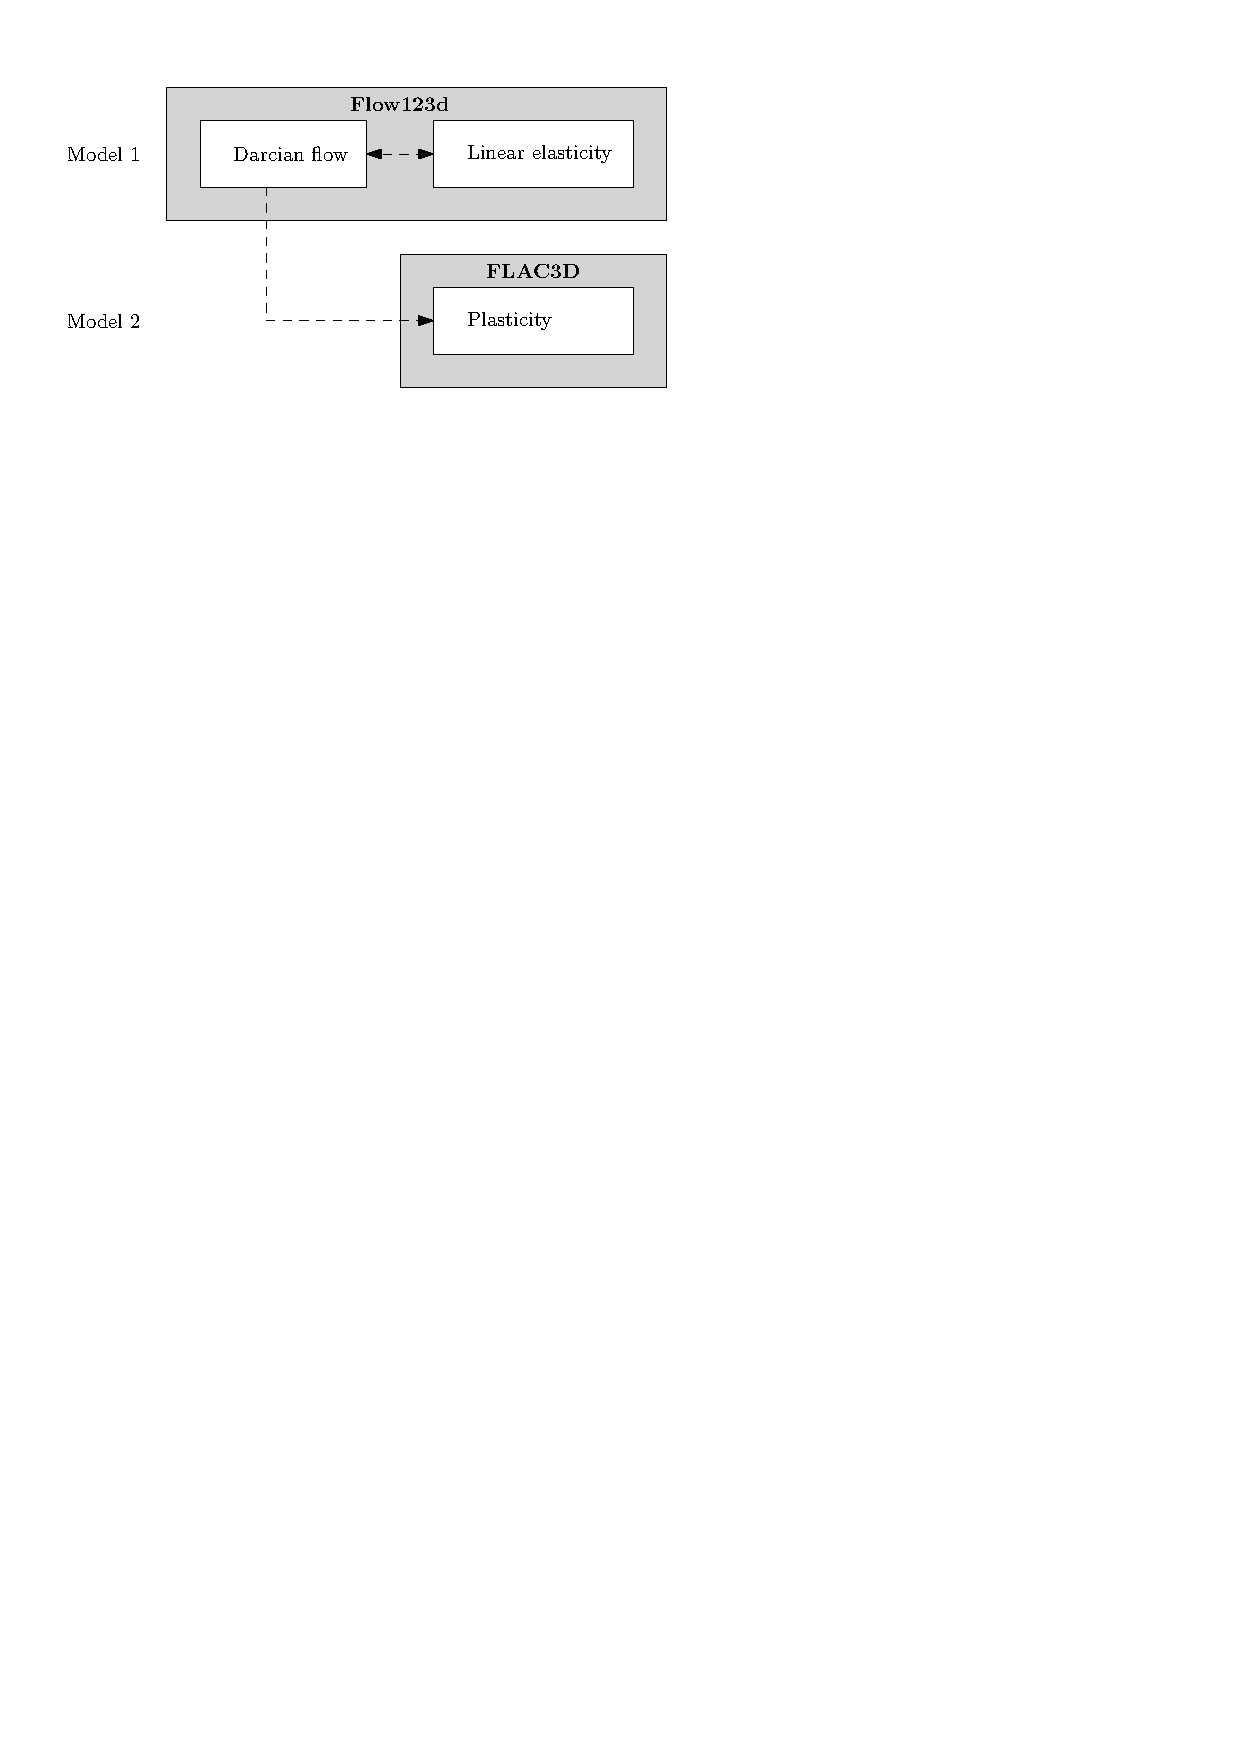
\includegraphics[width=0.75\textwidth]{graphics/comparison/sw_coupling.pdf}
    \caption{Overview of model coupling.}\label{fig:sw_coupling}
\end{figure}

% The extent of EDZ has generally a large impact on the permeability of the rock in the vicinity of excavations, and on the subsequent changes of pressure.
% To estimate the extent of EDZ and its impact on the pressure changes in rock mass, the poroelastic model developed using the Flow123d simulator was accomplished by a nonlinear mechanical model in FLAC3D.
The structure of the chapter is as follows. In Section \ref{sec:model_comparison} we describe the two models and report on their detailed comparison in the linear elastic case. This step was necessary to harmonize the settings of the two simulation models.
Next, Section \ref{sec:plasticity} is devoted to the results of Model 2 dealing with plasticity and EDZ.


\section{Linear elasticity - comparison of models}\label{sec:model_comparison}

\subsection{Description of models}

The area of interest is located around the laboratory gallery L5 in Bukov URF II, where two new test chambers, ZK5-1S and ZK5-1J were constructed.
The computational domain is a box with the dimensions $65\times50\times45$ \unit{\meter}, such that the X axis is in direction of the test chambers, the Y axis is oriented along the L5 gallery, and the Z axis is vertical.  The box center is located in the middle of the L5 gallery, in between the stationing of the test chambers ZK5-1S and ZK5-1J, with zero Z coordinate at the floor level,  see Fig. \ref{fig:model_geometry}.
\begin{figure}
    \centering
    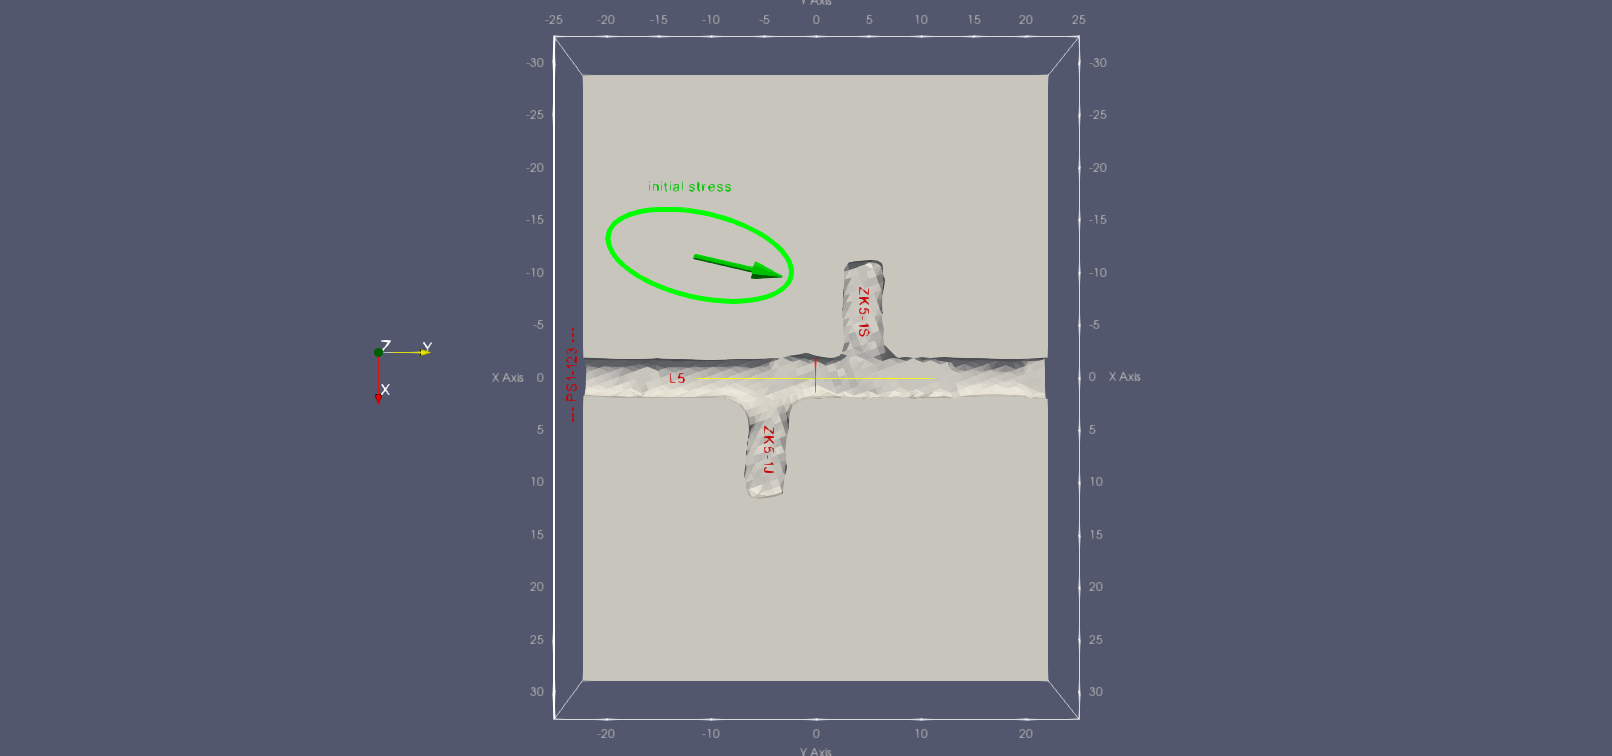
\includegraphics[width=\textwidth]{graphics/comparison/domain-z.png}
    \caption{Model geometry.}
    \label{fig:model_geometry}
\end{figure}

\paragraph{Model 1: poroelastic response to excavation.}
Model 1 describes the hydro-mechanical processes in rock mass during the excavation and in the subsequent relaxation period.
It is a slightly updated version of the model described in \cite{tz_design}.
The computational model is implemented using the Flow123d simulator, which supports the poroelastic coupling, but its mechanical part is limited to linear elasticity.

% The computational domain is a box $65\times50\times45$ \unit{\meter} with Y axis oriented along the gallery L5 and with the box center located at the floor level in the middle of the test chambers ZK5-1S and ZK5-1J.
The surface of the gallery L5 and of the two test chambers was obtained from laser scans.
The computational domain is fixed and consists of the box without the final shape of the excavations.

The hydro-mechanical model is described by the Biot equations:
\begin{equation}
\begin{aligned}
-\div\vc\sigma + \alpha\varrho_w g\nabla p &= \vc f,\\
\partial_t(S p+\alpha\div\vc u) + \div\vc v &= s,
\end{aligned}
\end{equation}
where $\vc\sigma$ is the effective stress tensor, $\alpha$ is the Biot-Willis coefficient, $\varrho_w$ is the water density, $g$ is the gravitational acceleration, $p$ is the pressure head, $\vc f$ is the load, $S$ is the storativity, $\vc u$ is the displacement, $\vc v$ is the Darcy flow velocity, and $s$ is the volume source of water.
We consider Hooke's and Darcy's laws as the constitutive relations for the stress tensor and velocity, respectively:
\begin{equation}
\vc\sigma - \vc\sigma_{0}=\tn C\vc\varepsilon(\vc u), \qquad \vc v = -\tn K(\nabla p+\vc g).
\end{equation}
Here $\vc\sigma_{0}$ is the initial stress and $\vc g$ is the gravity vector.
The elasticity tensor $\tn C$ and the hydraulic conductivity tensor $\tn K$ are given in terms of the Young modulus $E$ and the Poisson ratio $\nu$, and the hydraulic conductivity $k$, respectively.

The changes in hydraulic conductivity due to excavation are described by the formula
\begin{equation}\label{eq:conductivity_relation}
k(\vc\sigma) = \frac{\varrho_w g}{\mu_w} \left[
      \kappa_r + \kappa_\delta\exp\left(\log\left(\frac{\kappa_0 - \kappa_r}{\kappa_\delta}\right) \frac{\sigma_m}{\sigma_0}\right)
  \right] \exp\left(\gamma\frac{\max\{0,\sigma_{\mathrm{VM}c} - \sigma_c\}}{\sigma_c}\right),
\end{equation}
i.e. the hydraulic conductivity is affected by the mean stress $\sigma_m$, and the von Mises stress $\sigma_{VMc}$ (we refer to \cite{tz_design} for a detailed explanation of the formula \eqref{eq:conductivity_relation} and its parameters).

\paragraph{Parameter values, initial and boundary conditions.}
Following the review in Chapter \ref{chapter:review} and our previous considerations in \cite{tz_design}, we selected the values of model parameters (see Tab. \ref{tab:model_params} for their summary).
Below we give an explanation of the changes compared with the previous model.

While the real geology contains three separate materials, here we adopted a simplified approach by consolidating them into a single material.
The rock mass properties, namely the Young modulus and Poisson's ratio have been averaged from the values for amphibolites and migmatites (see Tab.~\ref{tab:hoek_brown_summary_improved}), namely we consider $E=72.5$ \unit\GPa~ and $\nu=0.215$.

% The parameter values are specified in Tab. \ref{tab:model_params}, see also \cite{tz_design}, Section 2.2.1 for their meaning. \sts{[S: Zde je vhodne dat do souvislosti parametry uvedene v tabulce \ref{tab:model_params} s parametry shrnutymi ve treti kapitole.]}

\begin{table}
\centering
\caption{Parameter values of Model 1.}
\label{tab:model_params}
\begin{tabular}{llcl}
    \toprule
    Name & Symbol & Value & Unit\\
    \midrule
    storativity & $S$ & $2.66\cdot10^{-7}$ & \unit{\per\meter}\\ % 9.81e3 * (3*(1-2*0.215)/72.5e9 + 0.007*5.1e-10)
    Young's modulus & $E$ & $72.5$ & \unit\GPa\\
    Poisson's ratio & $\nu$ & $0.215$ & \\
    Biot-Willis coefficient & $\alpha$ & $0.2$\\
    water density & $\varrho_w$ & $10^3$ & \unit{\kg\per\cubic\meter}\\
    water viscosity & $\mu_w$ & $10^{-3}$ & \unit{\pascal\second}\\
    in situ permeability & $\kappa_0$ & $3\cdot10^{-20}$ & \unit{\square\meter}\\
    residual permeability & $\kappa_r$ & $\kappa_0/33$ & \unit{\square\meter}\\
    stress-free permeability & $\kappa_\delta$ & $10^{-16}$ & \unit{\square\meter}\\
    stress-dependence factor & $\gamma$ & $6$\\
    stress threshold & $\sigma_c$ & $55$ & \unit\MPa \\
    \bottomrule
\end{tabular}
\end{table}

The in-situ stress measurements presented in Sec. \ref{sec:review_stress} show a large variability throughout \URFB.
Due to a strong heterogeneity and foliation patterns in the zone of interest, there is a significant uncertainty in the principal values and orientations.
We therefore use, in agreement with our previous study \cite{tz_design}, the values from hydrofrac tests in borehole L7-87D, namely the maximal and minimal horizontal stresses of $42$ \unit\MPa\ and $19$ \unit\MPa, respectively, and the vertical stress of $14$ \unit\MPa\ (see also \cite{tz_char_2}, p.~116).
The azimuth of the maximal stress is $123^\circ$, which means $13^\circ$ clockwise from the L5 axis.

During the initial water-pressure tests in the newly drilled boreholes in L5, a pressure of $400$ \unit\kPa\ was measured at a distance of $10$ \unit\meter\ from the gallery. Therefore, we use an initial piezometric head of $40$ \unit\meter\ before excavation.

On the outer box boundary, piezometric head $40$ \unit{\meter} and zero normal displacement is prescribed.
On the surface of L5 and of the excavated parts of the test chambers, zero pressure head and zero stress is prescribed.
The artificial boundary corresponding to not-yet excavated parts of the test chambers is subject to zero flux and initial stress.

Since the above-mentioned initial pressure condition is not compatible with the boundary condition on the tunnel walls, a period of 100 days prior to excavation was included in the simulation to allow the pressure field to relax toward a natural steady state.
Then a 30-day period of excavation was simulated, during which the boundary conditions were updated according to the excavation progress, see Fig. \ref{fig:excavation_progress}.
Finally, a 10-year period was simulated to track the relaxation of pore pressure in the rock mass.
\begin{figure}
    \centering
    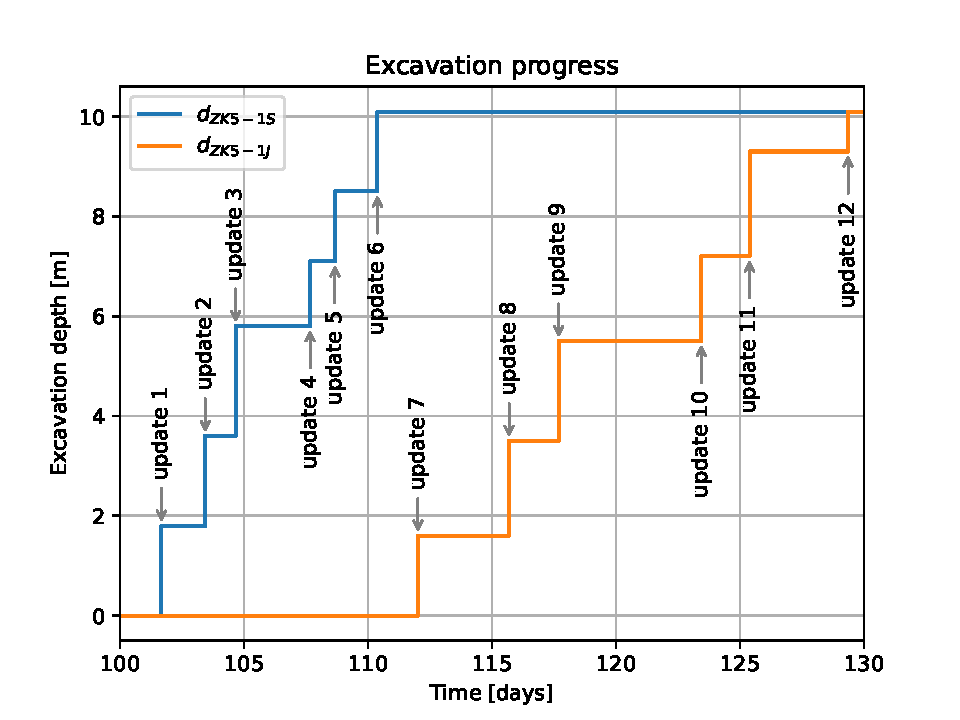
\includegraphics[width=\textwidth]{graphics/comparison/excavation_plot.pdf}
    \caption{Progress of excavation works on test chambers ZK5-1S and ZK5-1J.}
    \label{fig:excavation_progress}
\end{figure}


\paragraph{Model 2: mechanical response to excavation.}

Model 2 describes the mechanical response to the excavation.
It was implemented using the FLAC3D simulator, which does not provide hydraulics but offers more advanced mechanical models suitable for estimating the formation of EDZ, including plasticity criteria.
It takes the pore pressure field from Model 1 as an input and considers it as a volume load.
As the first step, a linear elastic case was investigated to find an equivalent parameter configuration with Model 1.

Model 2 is described in detail in Section \ref{sec:plasticity}.

Here we mention the principal differences to Model 1:
\begin{itemize}
    \item Model 2 computes the steady state mechanical response to excavation and to pressure field taken from Model 1, while Model 1 computes the time evolution of hydro-mechanical coupling.
    \item Model 2 uses computational meshes that are gradually updated according to the excavation progress with excavation modeled by weakening the cells and the surface mesh being a prescribed interior interface, while Model 1 uses a fixed computational mesh and time-dependent boundary conditions.
    \item The surface of the excavations is slightly regularized in Model 2, while in Model 1 the surface contains roughness as detected by laser scanning. Hence, the computational geometries are not identical.
    \item Model 2 uses computational meshes with approximately 311 thousand mainly hexahedral elements, while the mesh of Model 1 has 32 thousand tetrahedra.
\end{itemize}

In Fig. \ref{fig:model_surfaces} the surface meshes of both models are depicted.
\begin{figure}
    \centering
    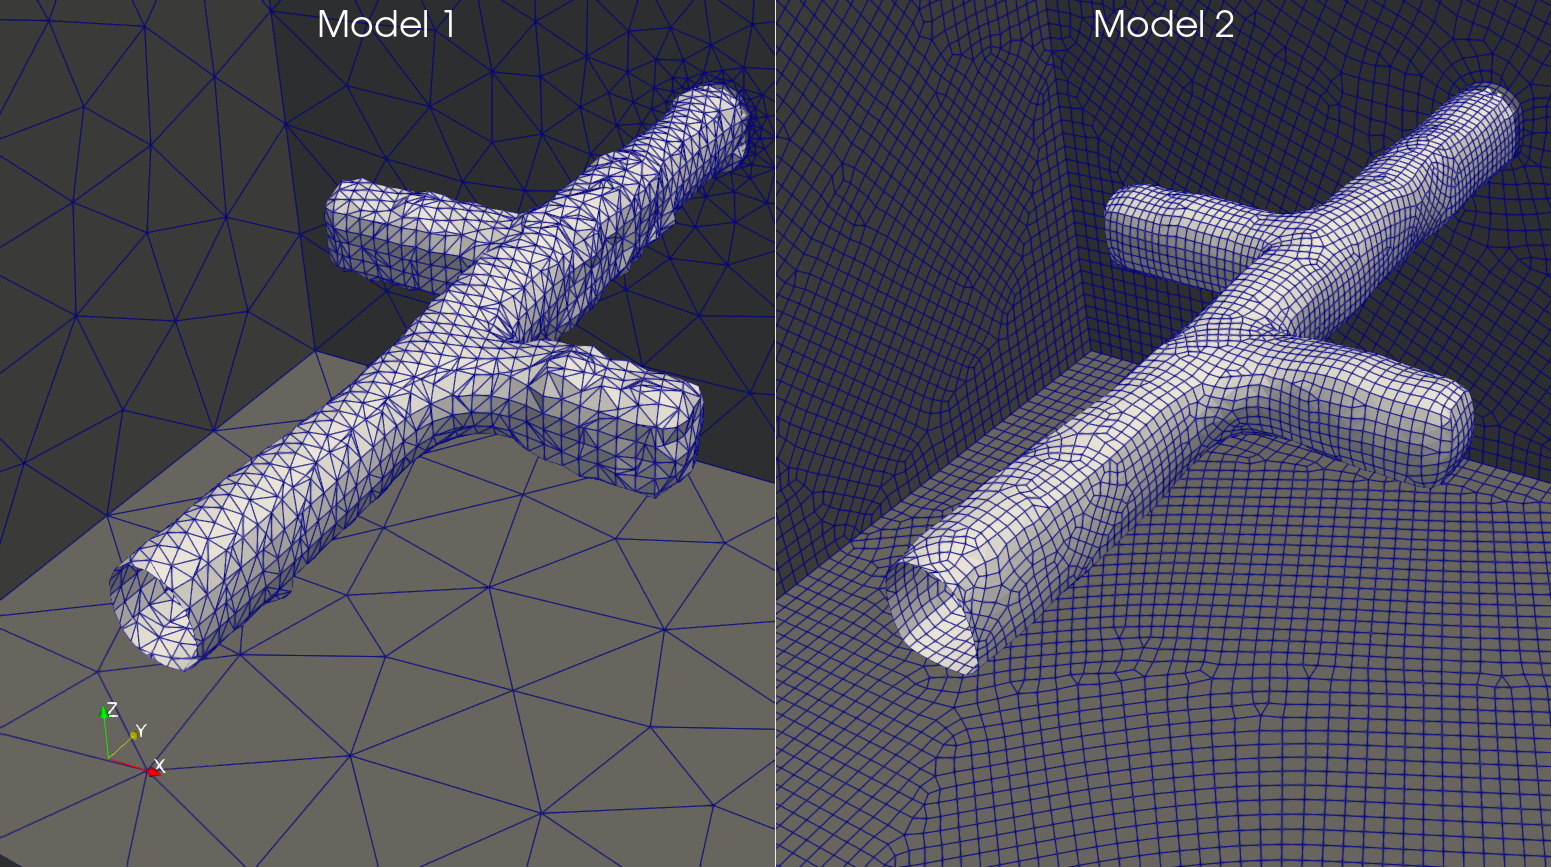
\includegraphics[width=\textwidth]{graphics/comparison/model_surfaces.png}
    \caption{Surface mesh of Model 1 (left) and Model 2 (right).}
    \label{fig:model_surfaces}
\end{figure}


\subsection{Comparison of models}

After several iterations of debugging the common parameter setup in the respective simulators,  Models 1 and 2 exhibited qualitative agreement in the computed displacement and stress fields.
The computational meshes were not identical, hence for a better assessment of the differences in results, further postprocessing had to be done.

\paragraph{Methodology.}

Since each model uses a different mesh and geometry of the excavations, a simple interpolation of results from one mesh to another was not meaningful.
To evaluate the differences in the results precisely, the following steps were performed.
\begin{enumerate}
    \item The mesh nodes of Model 1 on the excavated part of the surface were shifted to lie on the surface of Model 2. This does not guarantee a perfect match of both geometries, as parts of the shifted mesh 1 may still lie outside mesh 2.
    \item "Excavated" cells in mesh 2 were removed from the results.
    \item Displacement and stress fields from Model 1 were resampled onto mesh 2.
    \item Values which were not possible to resample in the previous step (because of their positions outside mesh 2) were extrapolated from nearest boundary.
    \item Difference in displacement and stress fields was  quantified in terms of the $L^2$-norm\footnote{The $L^2$-norm of a function $f$ in the domain $\Omega$ is defined as follows: $\|f\|_{L^2(\Omega)}^2 := \int_{\Omega}|f(x)|^2~dx$.}, e.g.
    \[ E_\uu(t):= \frac{\|\widetilde\uu^1(t)-\uu^2(t)\|_{L^2(\Omega_t)}}{\max\{\|\widetilde\uu^1(t)\|_{L^2(\Omega_t)},\|\uu^2(t)\|_{L^2(\Omega_t)}\}. } \]
    Here $\Omega_t$ stands for the rock domain in Model 2 at a given time $t$, $\widetilde\uu^1$ denotes the particular field (here displacement) from Model 1 mapped to mesh 2, and $\uu^2$ is the particular field from Model 2.
    \item Displacement and stress components were visualized 
    % on a clipped region 2 m above tunnel floor
    together with the absolute difference between models, and regions with mismatch larger than 10 \% of the maximal value of the particular field were detected.
\end{enumerate}


\paragraph{Results.}

The displacement and stress fields were evaluated in 14 time points corresponding to excavation phases.

The norm of overall differences in displacement and stress fields are shown in Fig. \ref{fig:displ_l2_norms} and Fig. \ref{fig:stress_l2_norms}, respectively.
\begin{figure}
    \centering
    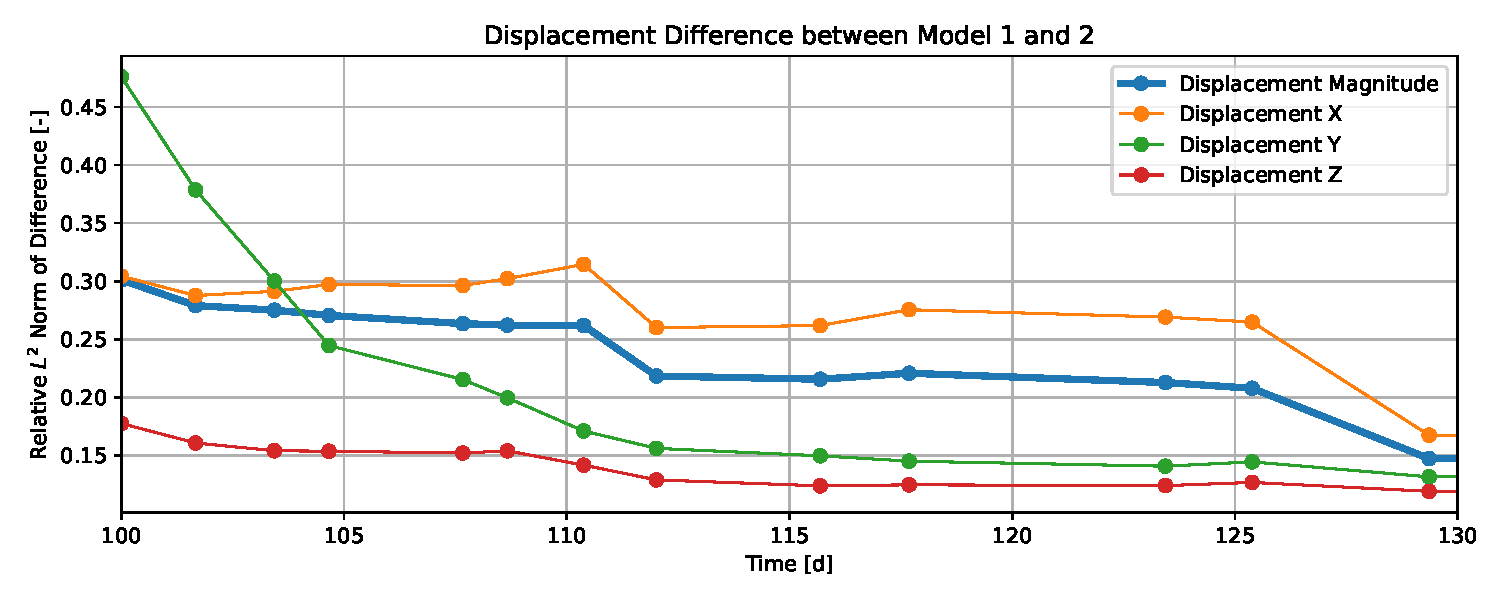
\includegraphics[width=\textwidth]{graphics/comparison/norms_displacement_diff_l2_norm_rel.pdf}
    \caption{Relative $L^2$ norm of differences between Model 1 and Model 2 for the displacement field and its components.}
    \label{fig:displ_l2_norms}
\end{figure}
\begin{figure}
    \centering
    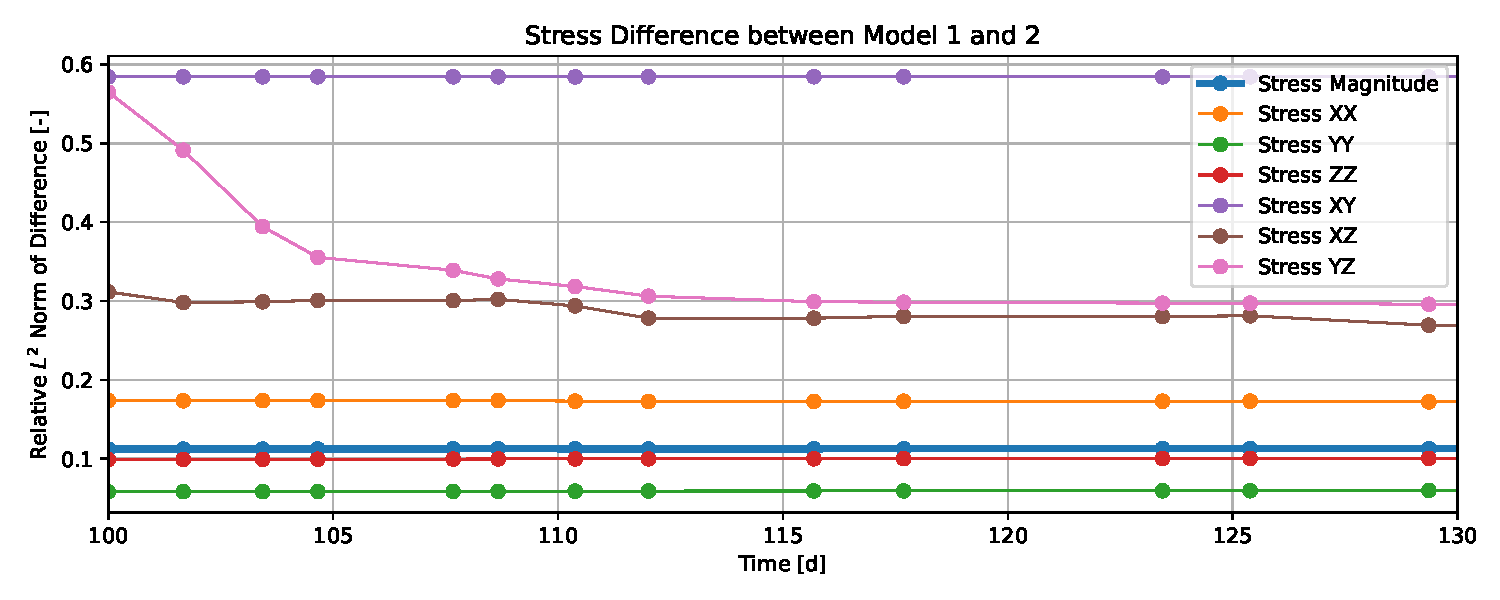
\includegraphics[width=\textwidth]{graphics/comparison/norms_stress_diff_l2_norm_rel.pdf}
    \caption{Relative $L^2$ norm of differences between Model 1 and Model 2 for the stress field and its components.}
    \label{fig:stress_l2_norms}
\end{figure}
One can observe that the differences in the whole displacement field are initially approximately 30 \% and drop to 15 \% after the 30 days of excavation.
Differences in the individual displacement components also generally diminish in time, although their initial mismatch differs (notably, the Y component has an initial relative mismatch of almost 50 \%).

Similarly, the relative norm of differences in the stress components is below 30 \%, with the exception of the YZ component (whose difference drops from 57 \% to 30 \% during excavation) and the XY component, whose difference remains close to 60 \%.
However, since the YZ and XY stress components are relatively small in absolute value, their significance to the overall stress difference is not large:
the difference in the whole stress field remains approximately 11 \% over time.

The 3D visualization of the differences provided additional insight and helped identify several sources of mismatch.
In what follows we summarize the main observations (note that the stress fields are visualized with the convention of compressive stress negative).
\begin{itemize}
    \item Except for the final time (update 13), significant differences are located around the not-yet-excavated parts of the two test chambers, where the Model 1 results were interpolated from distant cells. These differences disappear after the full chamber has been excavated. Hence, this mismatch is of limited importance. It is clearly visible, for example, in the X-displacement at update 6 (after ZK5-1S is excavated), see Fig. \ref{fig:comparison_displacements}.
    \begin{figure}[!htbp]
        \centering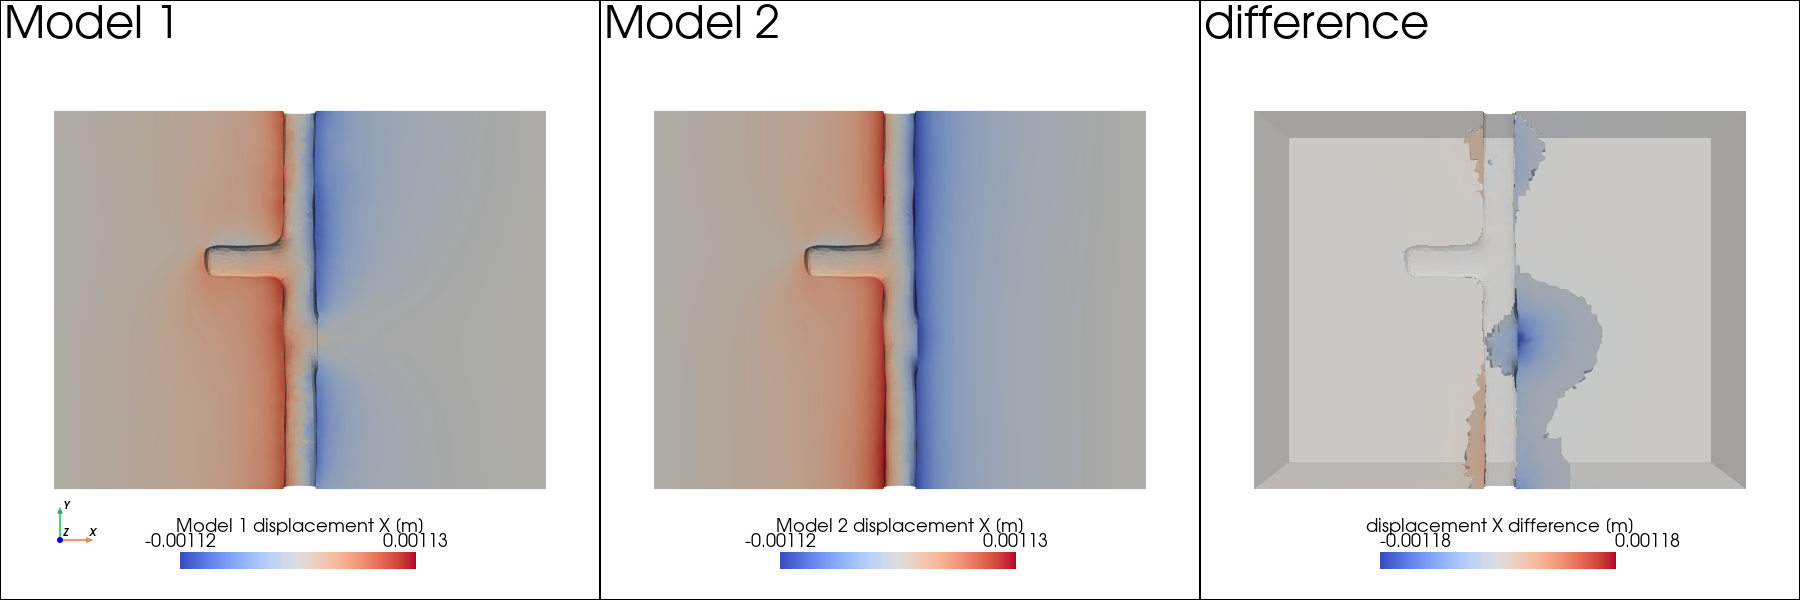
\includegraphics[width=\textwidth]{graphics/comparison/png-comparison/update_6_displacement-0.png}
        \caption{Difference between Model 1 and 2 in the X-component of the displacement (update 6).}\label{fig:comparison_displacements}
    \end{figure}

    \item The XX, YY, and ZZ components of stress have artificial singularities in the Model 2 results, which is a consequence of over-constrained displacement conditions. The resulting differences, however, remain located around the vertical edges of the outer box and do not affect the area of interest. See, for example, Fig. \ref{fig:comparison_stress_corners}.
    \begin{figure}[!htbp]
        \centering
        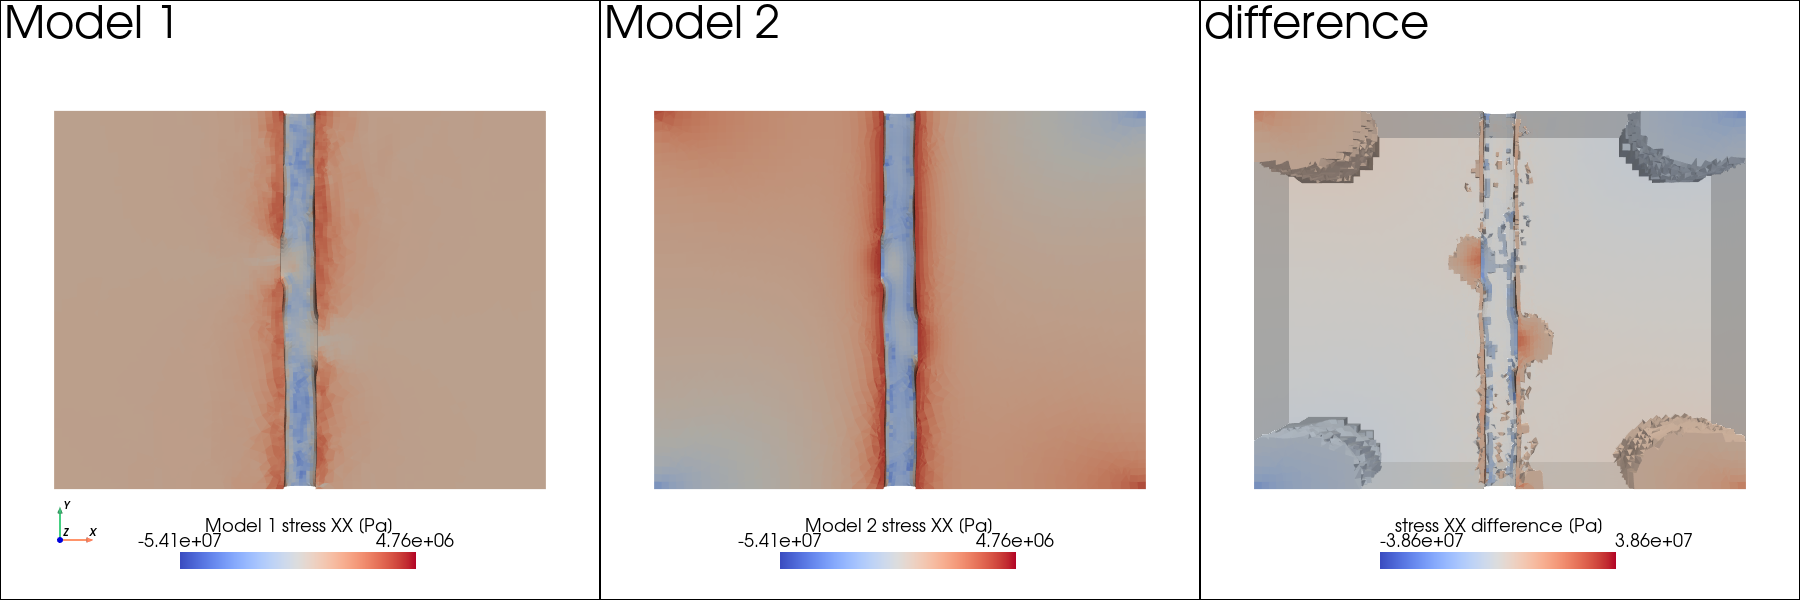
\includegraphics[width=\textwidth]{graphics/comparison/png-comparison/update_0_stress-0.png}
        \caption{Difference between Model 1 and 2 in the XX-component of the stress (update 0).}\label{fig:comparison_stress_corners}
    \end{figure}
    
    \item Probably the same reason underlies the difference in the shear XY component of stress, which, however, affects larger zones around the box boundary, including gallery L5. See Fig. \ref{fig:comparison_stress_xy}.
    \begin{figure}[!htbp]
        \centering
        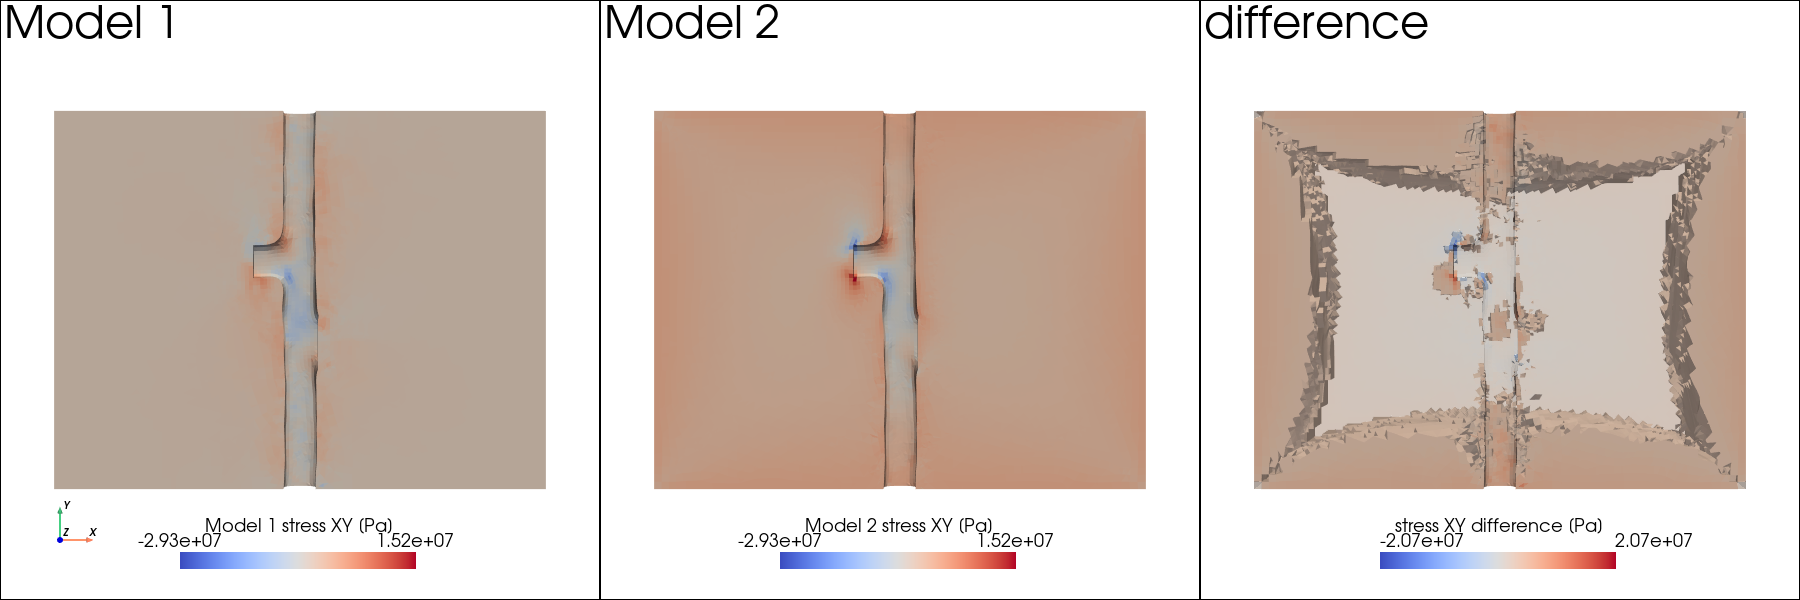
\includegraphics[width=\textwidth]{graphics/comparison/png-comparison/update_2_stress-3.png}
        \caption{Difference between Model 1 and 2 in the XY-component of the stress (update 2).}\label{fig:comparison_stress_xy}
    \end{figure}
    
    \item The differences in stress around points with extremal values are partly caused by interpolation error (during the resampling of Model 1 results, the values are slightly blurred, and therefore the extrema are lost). So the real difference (in case of using identical computational mesh) may be smaller. See Fig. \ref{fig:comparison_stress_yz}.
    \begin{figure}[!htbp]
        \centering
        \subfloat[Top view clipped at $z=2$ \unit\meter.]{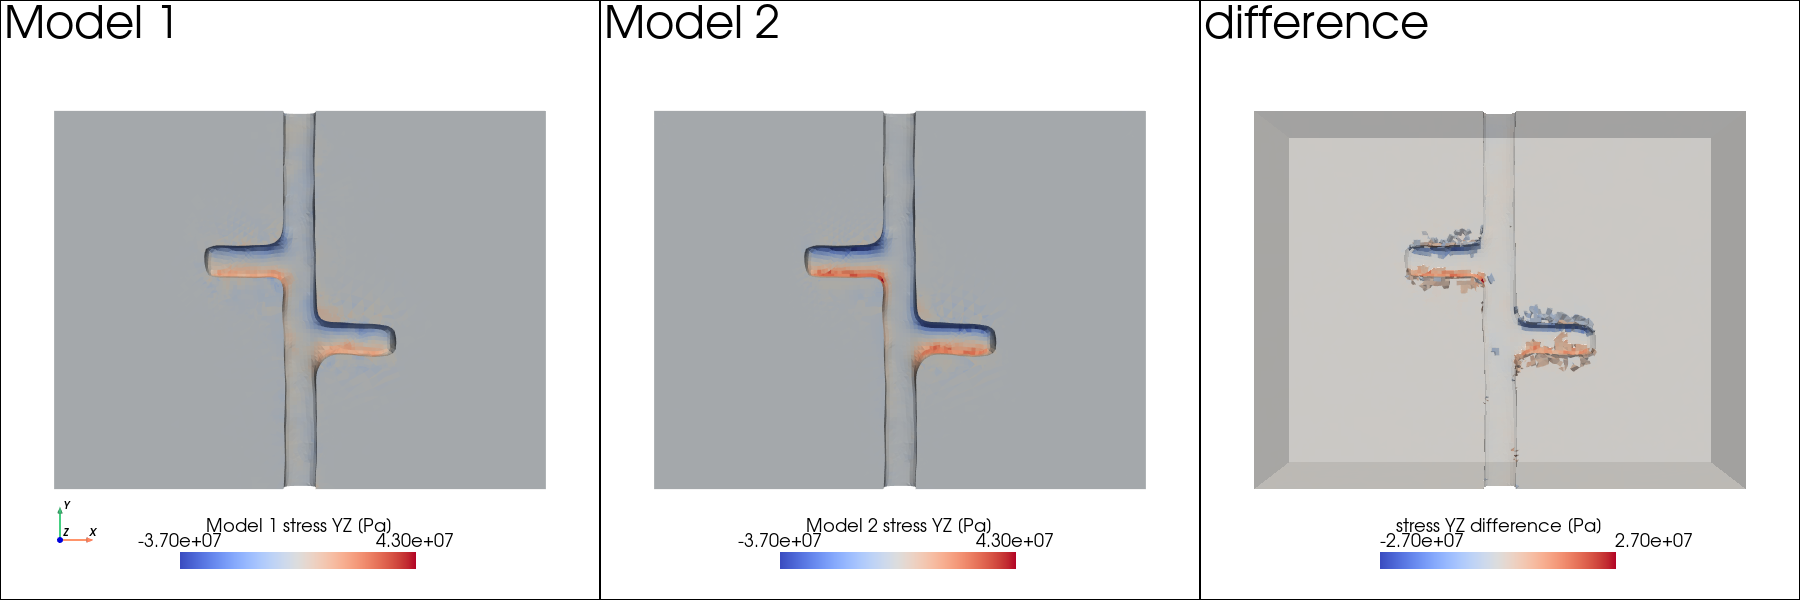
\includegraphics[width=\textwidth]{graphics/comparison/png-comparison/update_13_stress-5.png}}
        \hfill
        \subfloat[Side view clipped at $x=5$ \unit\meter. Influence of mapping onto different mesh.]{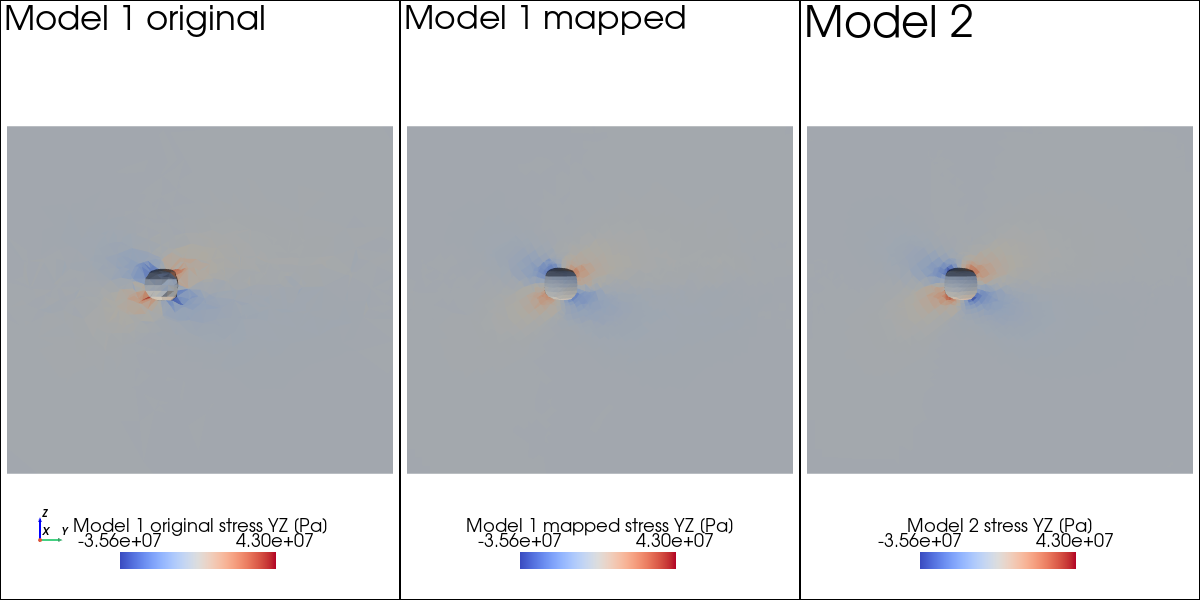
\includegraphics[width=\textwidth]{graphics/comparison/png-comparison/update_13_stress-5-mapped_clip_x.png}}
        \caption{Difference between Model 1 and 2 in the YZ-component of the stress in update 13.}\label{fig:comparison_stress_yz}
    \end{figure}
    
\end{itemize}


\subsection{Summary}

Two models of mechanical response to excavation and pore pressure changes were established and their parameters harmonized to give comparable results.
Detailed comparison of the results of both models revealed a good match, with the following major discrepancies:

\begin{itemize}
    \item Differences in the whole stress field (11 \%) are smaller than those in the whole displacement field (15--30 \%).
    In particular components, the mismatch is up to 60 \%.
    \item The differences diminish or stay constant in time.
    \item Some fundamental differences between Model 1 and 2 solvers were detected in the treatment of the boundary conditions and/or the initial stress.
    This presumably caused the largest discrepancies.
    \item Major discrepancies are located at the outer boundary, thus far enough from the zone of interest.
    \item Different treatment of excavation process leads to mismatch due to necessity to extrapolate values in the not-yet-excavated volume elements.
    \item Local differences in the vicinity of the excavations are caused mainly by interpolation error due to mapping of fields between models. The use of an identical mesh, or at least identical surface geometry in both models, would therefore be advantageous.

\end{itemize}
